%% start of file `template.tex'.
%% Copyright 2006-2013 Xavier Danaux (xdanaux@gmail.com).
%
% This work may be distributed and/or modified under the
% conditions of the LaTeX Project Public License version 1.3c,
% available at http://www.latex-project.org/lppl/.

\documentclass[11pt,a4paper,sans]{moderncv} % possible options include font size ('10pt', '11pt' and '12pt'), paper size ('a4paper', 'letterpaper', 'a5paper', 'legalpaper', 'executivepaper' and 'landscape') and font family ('sans' and 'roman')

% moderncv themes
\moderncvstyle{banking}                             % style options are 'casual' (default), 'classic', 'oldstyle' and 'banking'
\moderncvcolor{blue}    
 % color options 'blue' (default), 'orange', 'green', 'red', 'purple', 'grey' and 'black'
%\renewcommand{\familydefault}{\sfdefault}         % to set the default font; use '\sfdefault' for the default sans serif font, '\rmdefault' for the default roman one, or any tex font name
\nopagenumbers{}                                  % uncomment to suppress automatic page numbering for CVs longer than one page

% character encoding                      % if you are not using xelatex ou lualatex, replace by the encoding you are using
\usepackage[ngerman]{babel}
\usepackage[ansinew]{inputenc}
\usepackage[T1]{fontenc}
\usepackage[scale=0.75]{geometry}
\usepackage[leqno]{amsmath} 
\usepackage[]{ragged2e}
\usepackage{units}
\usepackage{eurosym}
%\usepackage{graphicx} dieses Paket kennt modern CV nicht. Darum arbeite besser mit einer Mini Page.
%\usepackage[Encodierer]{inputenc}
%\usepackage{CJKutf8}                              % if you need to use CJK to typeset your resume in Chinese, Japanese or Korean
% \makeatletter
% \@ifpackageloaded{moderncvstylebanking}{%
% \let\oldmakecvtitle\makecvtitle
% \renewcommand*{\makecvtitle}{%
%   {\centering\framebox{\includegraphics[width=\@photowidth]{\@photo}}\par\vspace{10pt}}%
%   \oldmakecvtitle%
%   
% }%
% }{%
% }
% \makeatother
% adjust the page margins
%\usepackage[scale=0.75]{geometry}
%\setlength{\hintscolumnwidth}{3cm}                % if you want to change the width of the column with the dates
%\setlength{\makecvtitlenamewidth}{10cm}           % for the 'classic' style, if you want to force the width allocated to your name and avoid line breaks. be careful though, the length is normally calculated to avoid any overlap with your personal info; use this at your own typographical risks...

% personal data
\name{Firstname}{Lastname}
\title{M.Sc.}                               % optional, remove / comment the line if not wanted
\address{Street 123}{4711 Town}{Country\medskip}% optional, remove / comment the line if not wanted; the "postcode city" and "country" arguments can be omitted or provided empty
%\phone[mobile]{049 151 22684134}                  % optional, remove / comment the line if not wanted; the optional "type" of the phone can be "mobile" (default), "fixed" or "fax"
\phone{+11 123456789}
%\phone[fax]{+3~(456)~789~012}
\email{email@host.com}                               % optional, remove / comment the line if not wanted
\homepage{www.google.com}                         % optional, remove / comment the line if not wanted
%\social[linkedin]{john.doe}                        % optional, remove / comment the line if not wanted
% \social[twitter]{jdoe}                             % optional, remove / comment the line if not wanted
% \social[github]{jdoe}                              % optional, remove / comment the line if not wanted
%\extrainfo{Geburtsdatum: 17.12.1989}                 % optional, remove / comment the line if not wanted
\photo[6,0cm][0.2pt]{bewerbungsbild.png}                      % optional, remove / comment the line if not wanted; '64pt' is the height the picture must be resized to, 0.4pt is the thickness of the frame around it (put it to 0pt for no frame) and 'picture' is the name of the picture file
% \quote{Some quote}                                 % optional, remove / comment the line if not wanted

% to show numerical labels in the bibliography (default is to show no labels); only useful if you make citations in your resume
%\makeatletter
%\renewcommand*{\bibliographyitemlabel}{\@biblabel{\arabic{enumiv}}}
%\makeatother
%\renewcommand*{\bibliographyitemlabel}{[\arabic{enumiv}]}% CONSIDER REPLACING THE ABOVE BY THIS

% bibliography with mutiple entries
%\usepackage{multibib}
%\newcites{book,misc}{{Books},{Others}}
%----------------------------------------------------------------------------------
%            content
%----------------------------------------------------------------------------------
\makeatletter
\@ifpackageloaded{moderncvstylebanking}{
\let\oldmakecvtitle\makecvtitle
\renewcommand*{\makecvtitle}{
  {\centering\framebox{\includegraphics[width=\@photowidth]{\@photo}}\par\vspace{10pt}}\oldmakecvtitle}}{}
\makeatother
\begin{document}
% #################################
% Cover Letter




\recipient{Company Name}{Street 123 \\ 4711 City \\ Country}
\date{\today}
\opening{\textbf{Application as Computer Programmer} \\\textsc{\scriptsize{Job-ID: 123456-789}}  \\ \vspace{0,5cm} Dear Ladies and Gentlemen, }
\closing{Best Regards \vspace{0,1cm} \\ 
\includegraphics[width=4.5cm]{unterschrift.png} \vspace{-1,5cm}}
\enclosure[Enclosure]{Curriculum vitae, certificates}           
%useanoptional argument to use a string other than "Enclosure", or redefine \enclname
\makelettertitle
\begin{justifying}

My several years of experience in converting requirements into logical flow charts, writing efficient and flawless programs and explain my code to technical and non technical peers might be an advantage for your company and increase your revenue. 
My several years of experience in [three most relevant keywords] might be an advantage for your company and increase your revenue. \newline

As a working student for company xyz I wrote several programs and created also logcial flow charts for sophisticated process in the area of xyz and released these programs to production. In the same role, I presented my programs and code in convincing and understandable way to external stakeholders as well as other programmers and created additional programming projects.
My documentation, which I have created with the tool xyz was used frequently and helped other programmers to understand my code and I updated my documentation ona daily basis.
I have also experience in tracking successfully inventory when I worked in a project for company xyz where we build up a inventory data base for more than 10 million different products using MS SQL database, Java as programming laguage and using workflow chart and diagram.\newline

This position fits well to my strenghts in the area of developing software, wirting documentation and I can apply my interest in modern IT topics as well as my experience in explaining complex programming strucutres in an understandbale way. My earlierst starting date is the 1st of January 2030 and my expected salary are 250.000 \$.

\bigskip
\end{justifying}

\makeletterclosing
% #################################
% CB......................
\newpage
\makecvtitle
\vspace{-1,0cm}
\section{Education}
%arguments 3 to 6 can be left empty
\cventry{04/13--03/16}{Master of Science}{University}{City}{\textit{Grade: 10,5}}{Physik}
\cventry{04/10--03/13}{Bachelor of Science}{University}{City}{\textit{Grade: 10,4}}{Physik}  


\section{Master Thesis}
\cvitem{Thema}{\emph{Research Name - Topic}, Grade: 10,0}
\cvitem{Supervisor}{Prof. Dr. Piguin, Dr. Jim Reynor}
\cvitem{Abstract}{Lorem ipsum dolor sit amet, consetetur sadipscing elitr, sed diam nonumy eirmod tempor invidunt ut labore et dolore magna aliquyam erat, sed diam voluptua. At vero eos et accusam et justo duo dolores et ea rebum. Stet clita kasd gubergren, no sea takimata sanctus est Lorem ipsum dolor sit amet. Lorem ipsum dolor sit amet, consetetur sadipscing elitr, sed diam nonumy eir.. }

\section{Bachelor Thesis}
\cvitem{Thema}{\emph{Research Name - Topic, Grade: 10,0}}
\cvitem{Betreuer}{Lorem ipsum dolor sit amet, consetetur sadipscing elitr, sed diam nonumy eirmod tempor invidunt ut labore et dolore magna aliquyam erat, sed diam voluptua. At vero eos et accusam et justo duo dolores et ea rebum. Stet clita kasd gubergren, no sea takimata sanctus est L.}
\newpage

% \section{Current Position}
% \cventry{10/07--12/07}{Name of Company}{Department}{Location}{}{
% Description what you are doing here...}
% 
% \section{Working Experience}
% \cventry{10/07--12/07}{Name of Company}{Department}{Location}{}{
% Description what you were doing here...}
% 
% \cventry{10/07--12/07}{Name of other Company}{Department}{Location}{}{
% Description what you were doing here...}

\section{Additional Qualifications}

\cventry{10/07--12/07}{Name of course}{Fun University}{Location}{}{
Description what you learned here}
\cventry{10/07--12/07}{Name of 2nd course}{Fun University}{Location}{}{
Description what you learned here...}

\section{Languages}
\cvdoubleitem{German}{Mother tongue}{English}{Fluent}{}
\cvitemwithcomment{French}{Basic Skills}{}

% \section{Sprachen}
% \cvdoubleitem{Deutsch}{Muttersprache}{Englisch}{Verhandlungssicher}{}
% \cvitemwithcomment{Deutsch}{Muttersprache}{}
% \cvitemwithcomment{Englisch}{Verhandlungssicher}{}
% \cvitemwithcomment{Franz�sisch}{Grundkenntnisse}{}
% \cvitemwithcomment{Portugisisch}{Grundkenntnisse}{}
\section{Tech Stack}
\cvdoubleitem{Office}{LaTeX}{Programming Laguage}{C++, Python}{}
\cvdoubleitem{Documentaton}{Jira, Confluence}{Logical Tools}{Flow Tool 1 ,Flow Tool 2}{}
\section{Personal Information}
\cvdoubleitem{Gender}{Male}{Nationality}{Pinguin Land}{}
\cvdoubleitem{Birth date}{11.\,11.\,1689}{Place of birth}{Pinguin Town}{}
% \cvline{Geburtsort}{Wiesbaden}{}
% \cvline{Nationalit�t}{Deutsch}{}
\cvline{Hobbies}{This and that}{}
\newpage
%\section{Referenzen}
%\cvitem{Prof. Dr.-Ing. habil. Tom Tuxer}{Fraunhofer Institut für Pinguinkunde, tom.tuxer@pingu.edu, (098)~7654~321}
% Publications from a BibTeX file without multibib
%  for numerical labels: \renewcommand{\bibliographyitemlabel}{\@biblabel{\arabic{enumiv}}}% CONSIDER MERGING WITH PREAMBLE PART
%  to redefine the heading string ("Publications"): \renewcommand{\refname}{Articles}
% \nocite{*}
\section{Certificates}
%oldstyle
\begin{minipage}{\textwidth}
  \centering
   %\hspace{-2.0cm}
  \includegraphics[width=.95\textwidth]{IMG_3181.jpg} \\
  Certificates, page 1
\end{minipage}
\newpage
\begin{minipage}{\textwidth}
  \centering
   %\hspace{-8.0cm}
  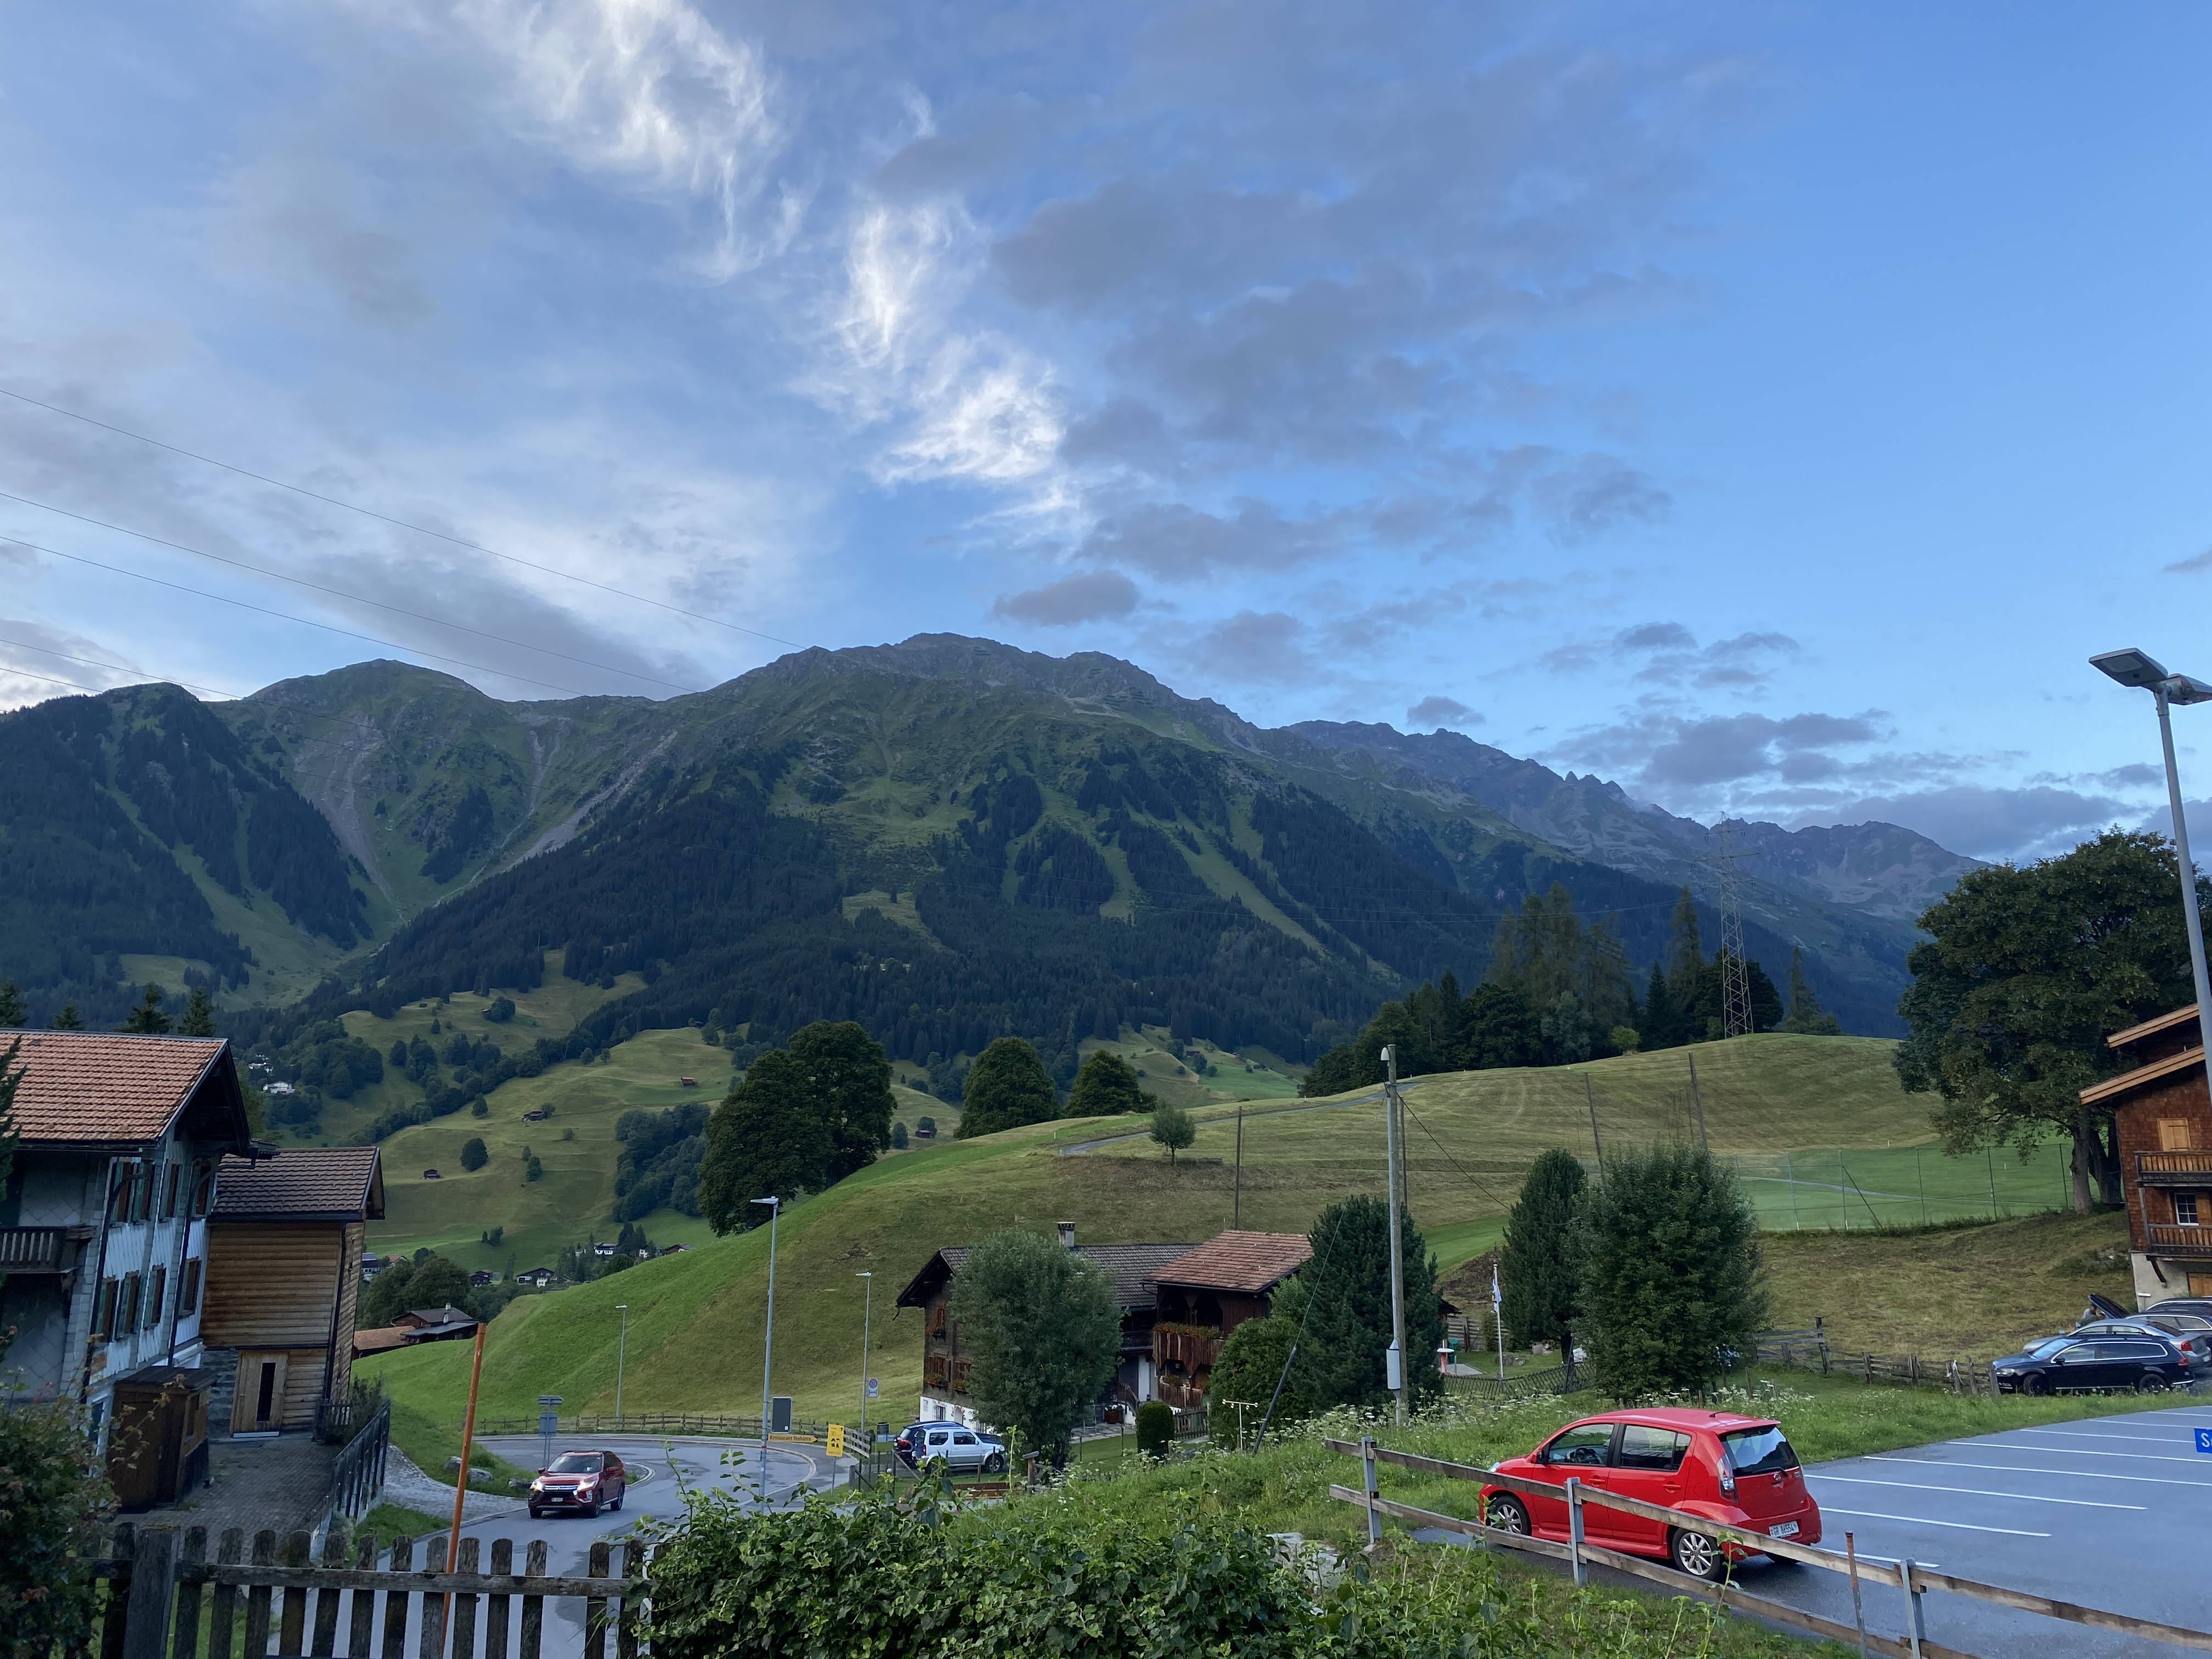
\includegraphics[width=0.95\textwidth]{IMG_3200.jpg} \\
  Certificates, page 2

\end{minipage}

\clearpage
\end{document}
%% end of file `template.tex'.
\grid
\grid
